\begin{usecase}{Continue with Google}
  \ucbasicinfo{High}{Regular}
  \ucshortdescription{This UC allows users to login or sign up with their Google account.}
  \uctrigger{This UC starts when the user clicks ``Continue with Google'' button in the app.}
  \ucactors{User}{Google}
  \ucpreconditions{The user must have an active Google account.}
  \ucrelationships{Send Welcome Email}{N/A}{N/A}
  \ucinputsoutputs{
    \begin{itemize}
      \item \textbf{Google access token} (Source: User)
    \end{itemize}
  }{
    \begin{itemize}
      \item \textbf{Authentication response} (Destination: User)
      \item \textbf{JWT} (Destination: App)
    \end{itemize}
  }
  \ucmainflow{
    \begin{enumerate}
      \item The user click continue with Google.
        \ucinfo{App uses OAuth to authenticate with Google}
      \item App sends Google access token to the system.
        \ucinfo{System verifies the token is issued for us and then issues JWT for usage within the app.}
    \end{enumerate}
  }
  \ucalternateflows{
    \begin{itemize}
      \item The user cancels the authentication request.
    \end{itemize}
  }
  \ucexceptions{
    \begin{itemize}
      \item Google access token invalid or expired.
      \item \textbf{Request sending failure}: If sending the request fails due to network issues, the system prompts the user to try again.
    \end{itemize}
  }
  \ucconclusion{This UC ends when the user is logged in.}
  \ucpostconditions{The system generates a JWT.}
  \ucspecialrequirements{A google client must be present for the validation of the access token to be possible.}
\end{usecase}

\begin{figure}[!h]
  \centering
  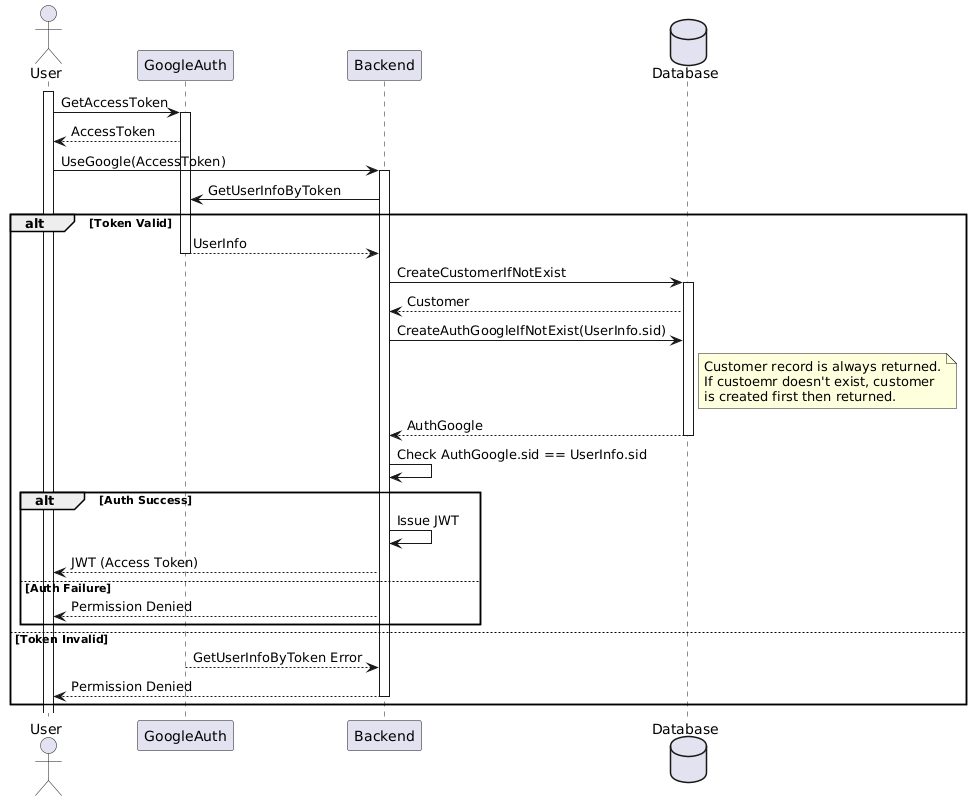
\includegraphics[width=\textwidth]{images/docs/diagrams/sequence-diagrams/all-sequence-diagrams/Continue with Google.png}
  \caption{Continue with Google Sequence Diagram}
  \label{fig:seq/continue-with-google}
\end{figure}

The "Continue with Google Sequence Diagram", shown in \textbf{Figure~\ref{fig:seq/Continue-with-Google }}, the user obtains an access token from GoogleAuth and shares it with the backend. The backend validates the token and retrieves user details through GoogleAuth. If the token is valid, the backend ensures the user exists in the database, creating a record if necessary, and associates the user’s Google account. It then verifies the session ID, issuing a JSON Web Token (JWT) for successful authentication or returning an error, such as Permission Denied, for invalid credentials. This process ensures secure and efficient authentication.